\documentclass[11pt,a4paper,oneside,onecolumn]{article}
\usepackage{amsmath}
\usepackage{fullpage}
\usepackage{color}
\usepackage{lastpage}
\usepackage{graphicx}
\usepackage{subfig}

\DeclareGraphicsExtensions{.png,.pdf} %pour pdflatex
\usepackage{multicol}
\usepackage{listings}
\usepackage{textcomp} %lettres grecques en texte


%\usepackage[latin1]{inputenc}%accents
%\usepackage[T1]{fontenc}
%\usepackage[francais]{babel}

%palatino
\usepackage[sc]{mathpazo}
\linespread{1.05}         % Palatino needs more leading (space between lines)


\usepackage[utf8]{inputenc}%accents
\usepackage[T1]{fontenc}
\usepackage[francais]{babel}
%\usepackage[french]{babel}

\usepackage[
pdfauthor={Olivier Bourrion},
pdftitle={MPPSYNC},
pdfsubject={MPPSYNC},
pdfkeywords={},
colorlinks={true},
linkcolor=red,
citecolor=green,
urlcolor=cyan,
pdfstartview={FitH}
]{hyperref}

%\DeclareTextFontCommand{\helvetica}{\fontfamily{phv}\selectfont}
%\renewcommand{\familydefault}{phv}

\usepackage{fancyhdr}
\setlength{\headheight}{15.2pt}
\pagestyle{fancyplain}
%\fancyhf{}
\headsep = 4pt
%%retrecissement header / footer
\voffset = -40pt
%\textheight = 609pt %default value
%\textheight = 729pt %default value
\addtolength{\textheight}{70pt}

\lhead{MPPSYNC}
\rhead{\today}
\lfoot{O. Bourrion}
\cfoot{\thepage\ of \pageref{LastPage}}

%%%%%%%%%%%%%%%%%%%%%%%%%%%%%%%%%%%%%%%%%%%%%%%%%%%%%%%%%%%%%%%%%%%%%%%%%%%%%%%%%%%%%%%%%%%%%%%%%%%%%%%%
\begin{document}
\vspace*{.5 cm}
\begin{center} {\Large Conception MPPSYNC} \end{center}
\vspace*{.5 cm}
%%%%%%%%%%%%%%%%%%%%%%%%%%%%%%%%%%%%%%%%%%%%%%%%%%%%%%%
\tableofcontents
%%%%%%%%%%%%%%%%%%%%%%%%%%%%%%%%%%%%%%%%%%%%%%%%%%%%%%%

\section{Spécifications}
\subsection{Demande pour polariseur et pour quart d'onde}
\begin{enumerate}
\item Boîtier autonome (prise 220\,V et contrôle par Ethernet et sorties pour pilotage moteur et lecteur capteur)
\item Synchronisation sur l'horloge externe de référence pour garder le synchronisme avec la DAQ.
\item Signal de start DAQ externe pour démarrer compteur interne ($2^{18}$) synchrone avec la DAQ sur horloge 250\,MHz, chaque tour de compteur un top\_DAQ a lieu (953\,Hz).
\item Avoir un moteur pas à pas pouvant tourner à 10\,tours/s, soit 1200\,tours/min.
\item Avoir un mode de recherche de zéro mécanique
\item Avoir un mode permettant de compter le nombre de pas pour faire un tour de polariseur.
\item Avoir un compteur de pas relatif, qui se remet à 0 après un nombre de pas déterminé (le nombre de pas par tour mesuré ou saisi).
\item Avoir un compteur de tour polariseur (incrémentation ou décrémentation), teste le capteur mécanique.
\item A chaque mesure DAQ (chaque 953\,Hz) pourvoir donner le nombre de pas effectué depuis la précédente remise à zéro du compteur de pas relatif.
%\item A chaque top capteur du 0, fournir l'état du compteur interne (mesure de déphasage et glissement par rapport à la DAQ).
\item Possibilité de faire avancer de \emph{n} degrés (ou pas) sur commande.
\item Le réglage de la fréquence de rotation du moteur doit pouvoir se faire en fraction réelle ($\frac{P}{Q}$) de la fréquence d'entrée.
\item Au niveau soft, être capable de configurer le nombre de pas moteur nécessaire pour faire un tour polariseur. (le tour polariseur dépend du facteur de réduction imposé par le rapport de courroie).
\item Pouvoir fixer la période de rotation du polarisation en définissant le nombre (entier) de top\_DAQ par tour.
\item Retourner un bit de status (chaque ms) indiquant si le moteur est en accélération, un autre si il est en rotation, arrêté). Un autre bit de status doit indiquer si le top 0 mécanique est bien arrivé au nombre de pas par tour de polariseur avec une fourchette d'acceptation réglable. Attention au sens de rotation
\item En mode rotation libre, prévoir un système permettant de laisser glisser le moteur (en le freinant ou l'accélérant pour avoir une phase donnée a chaque top\_synchro. 
Pour cela, il faut être capable d'indiquer au moteur de faire une vitesse de rotation donnée pour un nombre de pas donné (faiblement différente de la vitesse ciblée) puis dès que la première commande est terminée de retourner à la vitesse nominale (ou en pratique exécuter une deuxième commande chaînée).
Enchaînement de 2 commandes (bit de status pour commandes exécutées?)
\item Entrées du module (soft ou hard):
  \begin{itemize}
  \item Horloge de référence : 10\,MHz
  \item Signal start (TTL) en SMA
  \item 1 ou 2 signal de réserve
  \item Valeur P et Q pour régler la fréquence de défilement des pas
  \item Coefficient d'accélération
  \item Vitesse de rotation
  \item Réglage du courant moteur ?? Pour pouvoir mettre des moteurs plus petit
  \end {itemize}
  
\item Sorties du module (soft ou hard):
  \begin{itemize}
  \item Pilotage puissance du moteur
  \item Mesure capteur fourche optique (0 mécanique)
  \item Position angulaire du moteur utilisant le compteur relatif à 22\,Hz, soit avec une période de $\rm N \times top\_DAQ$ avec N programmable
  \item Durée entre fin cycle et top fourche optique (à 22\,Hz). Une méthode pratique pour mesurer cela est de faire tourner un compteur et de l'incrémenter jusqu'à ce que le capteur optique soit activé. La valeur de ce compteur est envoyé à chaque $\rm N \times top\_DAQ$, et remise à zéro. Elle permet ainsi d'obtenir une granularité fine sur l'instant de basculement du 0 mécanique entre 2 mesures.
  \item L'interface logicielle (mini PC) fabrique une trame de données tous les  N\_pt\_bloc (donc avec une période de $N\ top\_DAQ \times N\_pt\_bloc$) pour envoi par Ethernet.
  \item N\_pt\_bloc et N sont programmables (l'un agit sur le firmware et l'autre sur le logiciel PC)
  \end {itemize}
  
\end{enumerate}

\section{Solution utilisée}
\subsection{Quelques rappels}
La fréquence de rotation d'un moteur se fixe par :
\begin{equation}
 \omega=\dfrac{P}{Q}*RefClock  \times \dfrac{NbPasMoteurParTour}{NbPasParImpulsion}=f_{step} \times \dfrac{NbPasMoteurParTour}{NbPasParImpulsion}
\end{equation}
Où:
\begin{itemize}
 \item \textbf{$\omega$} est la vitesse de rotation en tour par seconde
 \item \textbf{P} est une valeur réglable de 0 à Q.
 \item \textbf{Q} est une valeur réglable de 0 à $2^{18}$ (en fonctionnement a 250\,MHz).
 \item \textbf{NbPasMoteurParTour} est le nombre de pas moteur par tour (donnée constructeur).
 \item \textbf{NbPasParImpulsion} est le nombre de pas effectué pour chaque impulsion envoyé au contrôleur de puissance. Cela est nécessaire dans le cas d'une utilisation, demi, quart ou micro pas.
\end{itemize}

Il faut aussi gérer l'accélération et la décélération du moteur. Elle se fera par une une constante pour incrémenter ou décrémenter la fréquence $f_{step}$ et donc la vitesse de rotation. A priori on gérera des valeur de variation de 4000\,Hz/sec à 500\,kHz/s.

Le système de réglage de fréquence estsur le même principe que les accumulateurs de phases dans NIKEL, la seule différence est que le compteur est borné jusqu’à Q pour pouvoir faire des fractions réglable. 
Pour chaque accumulation il faut vérifier que le max n'est dépassé, et si il l'est il faut ajouter le reliquat du dépassement à zéro.

%%%%%%%%%%%%%%%%%%%%%%%%%%%%%%%%%%%%%%%%%%%%%%%%%%%%%%%%%%%%%%%%%%%%%%%%%%%%%%%%%
\subsection{Vue générale du cœur du contrôleur  moteur}
La fréquence du moteur est générée par un compteur à \emph{n} bit. Cela permet une résolution fréquentielle qui est donnée par $\frac{f}{2^n}$. Une vue schématique du contrôleur est donnée à la figure~\ref{MPPSYNC_general}. On peut y voir une machine d'état qui est charge de gérer les diverses variation de vitesse du moteur, elle contrôle le pas d'incrémentation (\emph{frequency\_increment}). Son fonctionnement est détaillé par la suite dans la section~\ref{speedFSM_sec}.
\begin{figure}[th]
\begin{center}
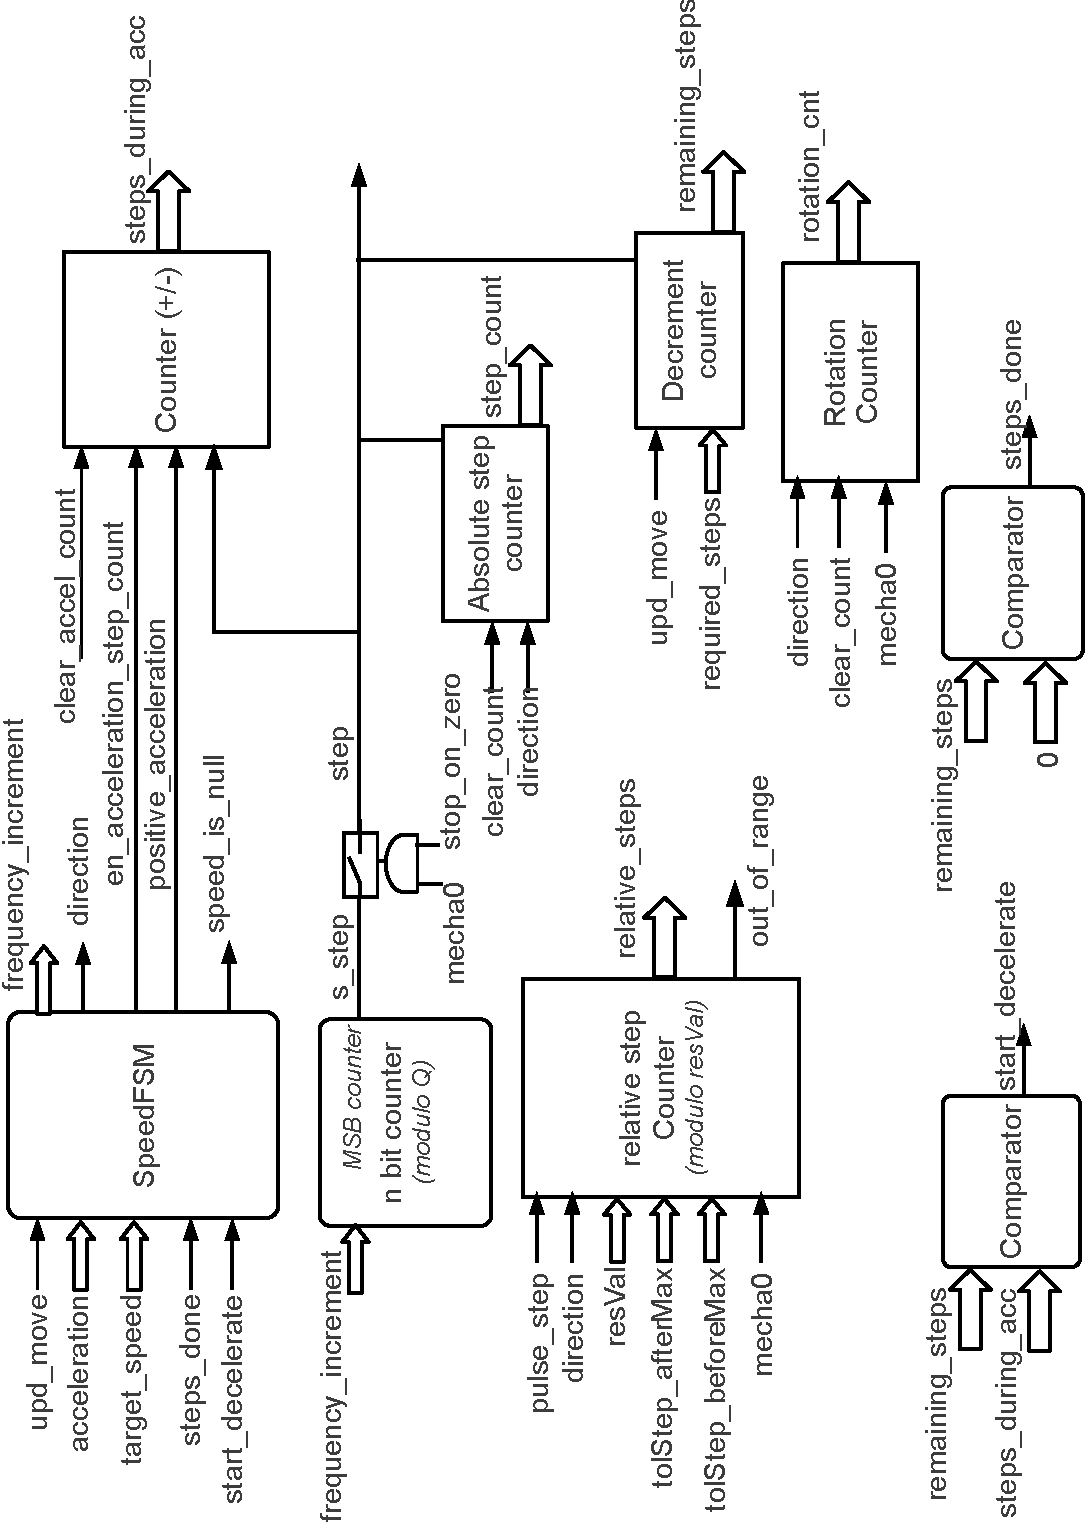
\includegraphics[angle=-90,width=\textwidth]{./figs/MPPSYNC_general}
\caption{Vue générale du cœur du contrôleur  moteur.}
\label{MPPSYNC_general}
\end{center}
\end{figure}
D'autres compteurs sont implémentes:
\begin{itemize}
 \item Un compteur de pas absolu, qui peut être remis à zéro à tout moment par le contrôle commande.
 \item Un compteur de pas relatif, qui peut être remis à zéro aà chaque fois qu'il atteint \emph{resVal}. En réglant \emph{resVal} au nombre de pas par tour de polariseur on peut vérifier a chaque tour si le nombre de pas observé est bien dans la fourchette de tolérance programmée (\emph{tolStep}). Si ce n'est pas le cas un flag est activé. Ce compteur doit pouvoir gérer les 2 sens de rotation.
 \item Un compteur de pas restant à faire, ce qui sert à effectuer un mouvement d'un nombre de pas donné. Si la valeur programmée est égale au maximum, on considère que c'est un déplacement libre illimité.
 \item Un compteur de pas en phase d'accélération, qui sert à estimer le nombre de pas nécessaire à une décélération maîtrisée. Ce compteur est incrémenté ou décrémenté en fonction du signe de l'accélération. 
\end{itemize}

Pour effectuer une recherche du zéro mécanique, le bit \emph{stop\_on\_zero} est activé et le moteur est lancé en rotation libre a faible vitesse. 
Il se stoppe tout seul lorsque le zéro mécanique est trouvé.

Partant de cet état, il est possible de compter le nombre de pas requis pour faire un tour de polariseur.
Il suffit de relancer la procédure de recherche de zéro après avoir fait une remise à zéro du compteur de pas absolu, et d'aller lire la valeur de compteur une fois le nouveau retrouvé.


%%%%%%%%%%%%%%%%%%%%%%%%%%%%%%%%%%%%%%%%%%%%%%%%%%%%%%%%%%%%%%%%%%%%%%%%%%%%%%%%%
\subsection{FSM de gestion de l'accélération moteur}
\label{speedFSM_sec}
La machine d'état (FSM) qui se trouve en figure\,\ref{MPPSYNC_speed_FSM} résume les divers étapes à traverser. elle permet de gérer des changement de direction et de consigne de vitesse à partir de n'importe quel état. En mode, nombre de pas fini, l'information du nombre de pas passé en accélération (ce nombre est décrémenté en décélération) est utilisé pour savoir quand démarrer la décélération. Celle-ci se poursuit jusqu'à la vitesse mini programmée. Puis partant de là, dès que le nombre de pas est atteint le moteur est stoppé. Cela sert à garantir que si il y a une erreur sur l'estimation du nombre de pas de freinage (en minorant), on fera au moins suffisamment de pas pour atteindre la consigne.
\begin{figure}[th]
\begin{center}
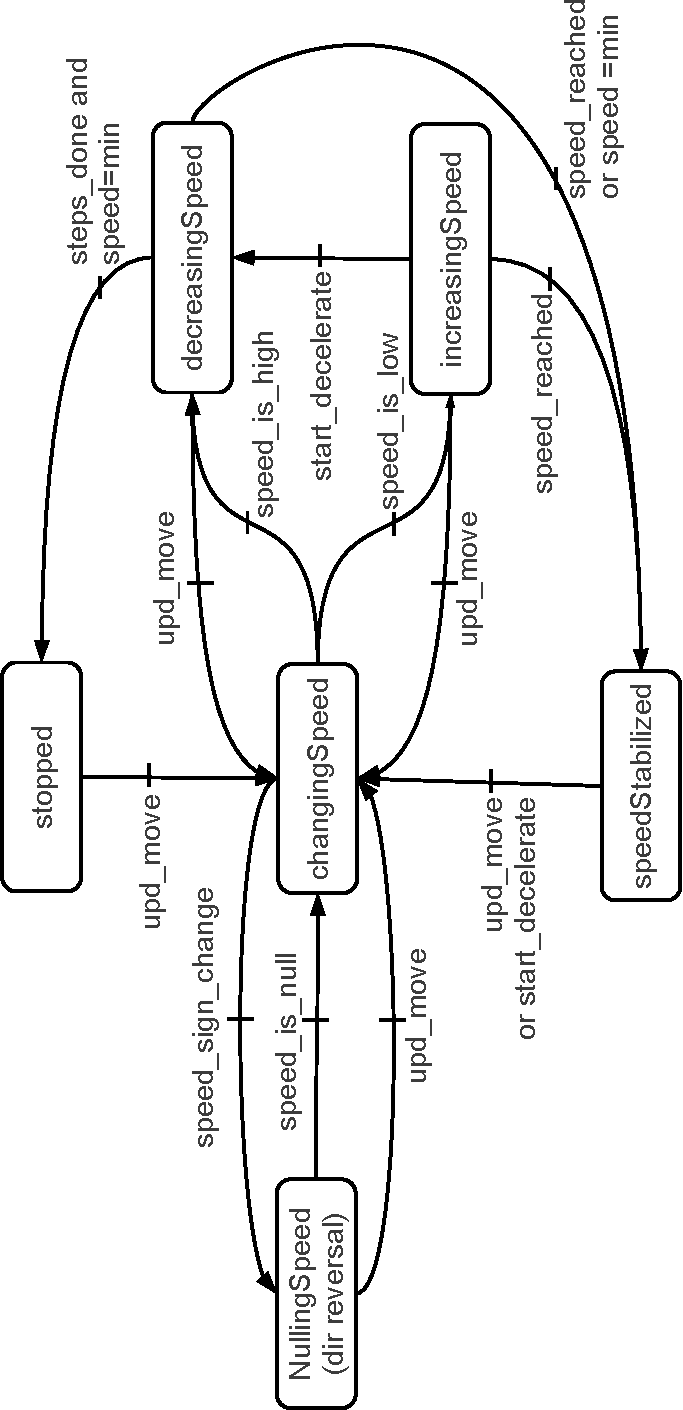
\includegraphics[angle=-90,width=\textwidth]{./figs/MPPSYNC_speed_FSM}
\caption{FSM de gestion de l'accélération moteur.}
\label{MPPSYNC_speed_FSM}
\end{center}
\end{figure}
Si la consigne du nombre de pas ou de vitesse change pendant qu'une autre consigne est en exécution, celle est court est avortée et aussi il se peut que plus de pas soient parcouru que demandé pour garantir une décélération correcte. Le paramètre de décélération ne peut être changé que en mode \emph{stopped}.

La vitesse de rotation est changée chaque micro-seconde en fonction du paramètre d'accélération.

Dans le cas d'un changement de sens de rotation le passage par une vitesse nulle est obligatoire avant de changer le sens de rotation.

Si le nombre de pas demandé ne permet pas une décélération correcte, le respect de la rampe de décélération imposera que le nombre de pas effectué en réalité sera plus grand et ne respectera pas la consigne. Cela peut arriver dans le cas d'une succession de deux commandes, alors que la première est toujours en cours. Par exemple, une demande de déplacement significativement plus faible alors qu'une précédente commande toujours en cours a permis au moteur d'atteindre la pleine vitesse. 

La figure~\ref{MPPSYNC_speedProfiles} donne quelques profils de vitesse en fonction des situations.
\begin{figure}[th]
\begin{center}
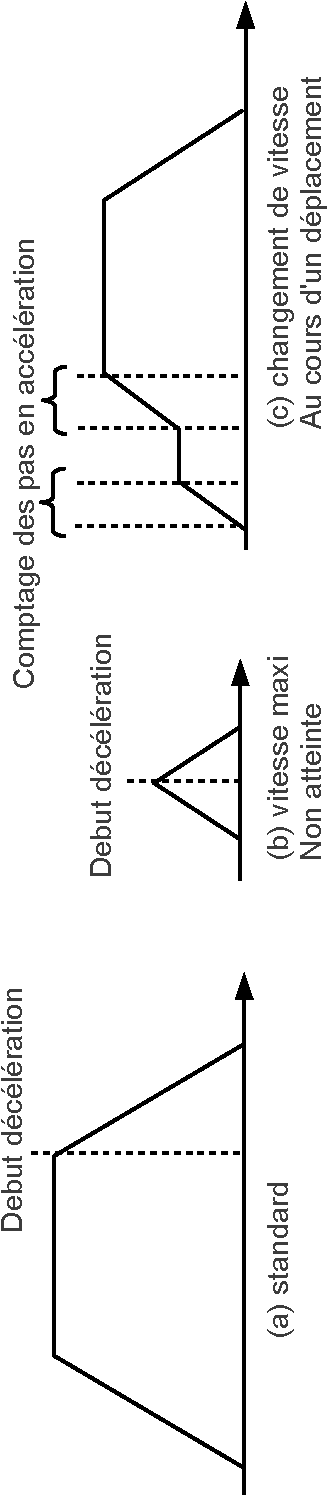
\includegraphics[angle=-90,width=\textwidth]{./figs/MPPSYNC_speedProfiles}
\caption{Exemple de profils de vitesse en fonction du temps. Le cas standard (a), le cas (b) où la vitesse maximum n'est pas atteinte quand la décélération doit déjà commencer et enfin le cas (c) qui montre pendant quelles parties le compteur de pas en phase d'accélération est modifié (ici le cas de accélération successives est illustré).}
\label{MPPSYNC_speedProfiles}
\end{center}
\end{figure}

%%%%%%%%%%%%%%%%%%%%%%%%%%%%%%%%%%%%%%%%%%%%%%%%%%%%%%%%%%%%%%%%%%%%%%%%%%%%%%%%%
\subsection{FSM de gestion des commandes}
Deux modes de commande sont prévus:
\begin{itemize}
 \item La commande standard, à exécution immédiate, et qui comprend une seule consigne de déplacement.
 \item La commande chaînée, qui ne s'exécute en deux parties et qui attend la fin de l'exécution de la première partie avant de lancer la deuxième. Elle sera utilisée principalement pour faire les recalages de phase lors du mode à rotation continue. Cela signifie, que lors de l'exécution de la première commande qui sera toujours une consigne d'un nombre de pas à vitesse connue et faiblement différente de la vitesse nominale, il n'y aura pas de phase de décélération vers un arrêt moteur, mais toujours une deuxième consigne qui suit et qui indiquera une vitesse de rotation différente pour un nombre de pas infini.
\end{itemize}


La FSM a donc deux files de commande, une pour les commandes standards et une pour les commandes chaînées. 
A chaque arrivée de nouvelle commande, l'exécution en cours est interrompue et la nouvelle commande est acceptée.
La figure~\ref{MPPSYNC_command_FSM} décrit le fonctionnement de la FSM de gestion des commandes. il est à noter que les commandes reçue via USB passent par cette FSM et que évidemment le sens de rotation ne peut pas changer entre les 2 parties de la commande chaînée. Une commande standard étant à exécution immédiate, il est impossible de demander une autre commande pendant que celle ci-est en exécution.

\begin{figure}[th]
\begin{center}
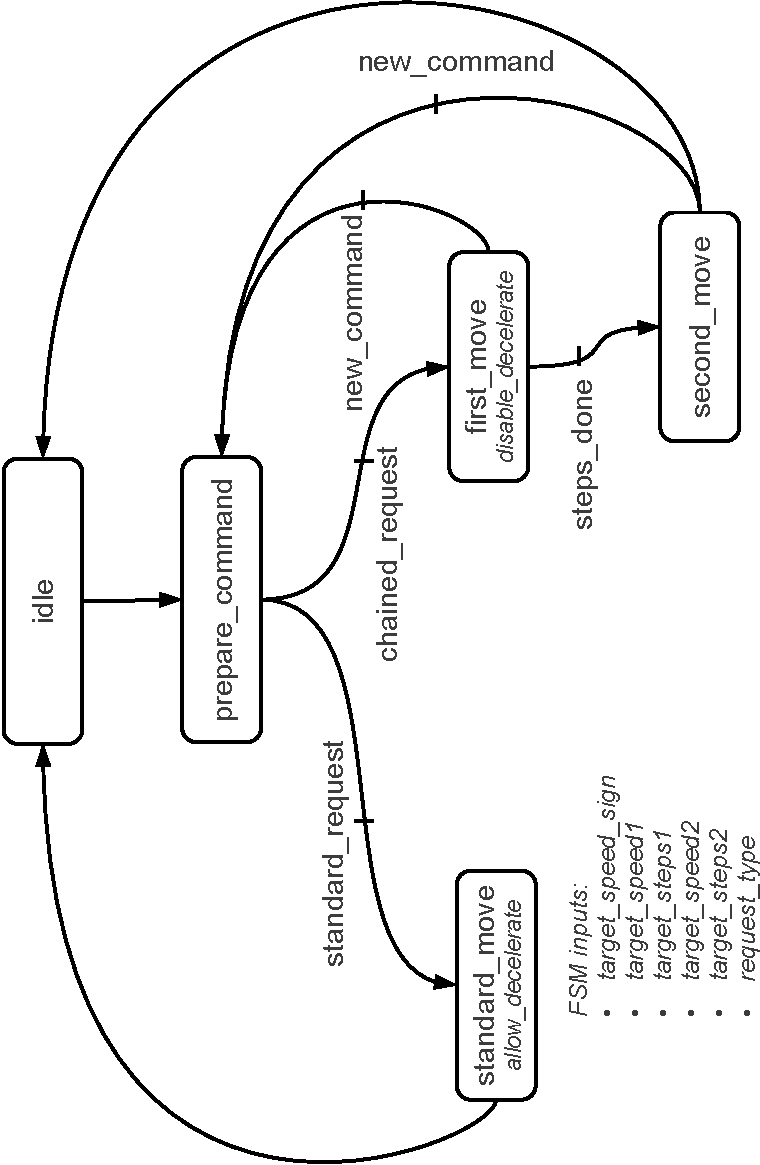
\includegraphics[angle=-90,width=0.8\textwidth]{./figs/MPPSYNC_command_FSM}
\caption{FSM de gestion des commandes moteurs.}
\label{MPPSYNC_command_FSM}
\end{center}
\end{figure}

%%%%%%%%%%%%%%%%%%%%%%%%%%%%%%%%%%%%%%%%%%%%%%%%%%%%%%%%%%%%%%%%%%%%%%%%%%%%%%%%%
\section{Calculs pour la synchronisation de la vitesse moteur avec la DAQ}
Le but est d'obtenir un nombre exact d'acquisition (faite par les boitiers NIKEL) pour chaque rotation du polariseur. Rappels:

\begin{equation}
 F_{DAQ}=\dfrac{250\,MHz}{2^{18} \times \_div\_KID}
\end{equation}
Où :
\begin{itemize}
 \item [$F_{DAQ}$] est la fréquence des données NIKEL
 \item [$\_div\_KID$] Nombre de données NIKEL a environ 1\,kHz pour faire un jeu de données
\end{itemize}

\begin{equation}
 F_{step}=\dfrac{50\,MHz}{Q} \times V
\end{equation}
Où :
\begin{itemize}
 \item [$F_{step}$] est la fréquence des pas en Hz
 \item [$Q$] est le diviseur de fréquence
 \item [$V$] est la valeur de vitesse (en bin) choisie
 \end{itemize}

 \begin{equation}
 F_{tour}=F_{step} \times \dfrac{1}{NbPasMoteurParTour}= \dfrac{50\,MHz}{Q} \times V \times \dfrac{1}{NbPasMoteurParTour}
\end{equation}
Où :
\begin{itemize}
 \item [$F_{step}$] est la fréquence des pas en Hz
 \item [$Q$] est le diviseur de fréquence
 \item [$V$] est la valeur de vitesse (en bin) choisie
 \item [$NbPasMoteurParTour$] est le nombre de pas moteur par tour (dépendant du mode micro-pas).
 \end{itemize}
 
Du coup, on peut exprimer le nombre de mesure par tour en faisant :
 \begin{equation}
 F_{DAQ}/F_{tour}=\dfrac{\dfrac{250\,MHz}{2^{18} \times \_div\_KID}} {\dfrac{50\,MHz}{Q} \times V \times \dfrac{1}{NbPasMoteurParTour}}
 =\dfrac{5 \times Q \times NbPasMoteurParTour}{2^{18}  \times \_div\_KID \times V}
\end{equation}
 
En exprimant la vitesse à régler en fonction du nombre de mesure par tour désiré, et en remplaçant $\dfrac{F_{DAQ}}{F_{tour}}$ par $N_{meas}$ :
 \begin{equation}
 V= \dfrac{5 \times Q \times NbPasMoteurParTour}{2^{18}  \times \_div\_KID \times N_{meas}}
\end{equation}

Application numérique avec $Q=2^{24}$, $\_div\_KID=40$ et $NbPasMoteurParTour=51200$ :
 \begin{equation}
 V= \dfrac{5 \times 2^{24} \times 51200}{2^{18}  \times 40 \times N_{meas}}= \dfrac{5 \times 2^{6} \times 1280}{N_{meas}}=\dfrac{25 \times 2^{14}}{N_{meas}}
\end{equation}

soit pour :
\begin{itemize}
 \item [$N_{meas}=50$] V=8192
 \item [$N_{meas}=100$] V=4096
\end{itemize}

\end{document}

